% Lab 9  for ENGR 1120 020 120 - Tristan Hill - Fall 2016 - Spring 2018 - Spring 2020
% 
% Introduction to MATLAB 
%
%  

% Document settings
\documentclass[11pt]{article}
\usepackage[margin=1in]{geometry}
\usepackage[pdftex]{graphicx}
\usepackage{multirow}
\usepackage{setspace}
\usepackage{hyperref}
\usepackage{color,soul}
\usepackage{fancyvrb}
\usepackage{framed}
\usepackage{wasysym}
\usepackage{multicol}

\pagestyle{plain}
\setlength\parindent{0pt}
\hypersetup{
    bookmarks=true,         % show bookmarks bar?
    unicode=false,          % non-Latin characters in Acrobat’s bookmarks
    pdftoolbar=true,        % show Acrobat’s toolbar?
    pdfmenubar=true,        % show Acrobat’s menu?
    pdffitwindow=false,     % window fit to page when opened
    pdfstartview={FitH},    % fits the width of the page to the window
    pdftitle={My title},    % title
    pdfauthor={Author},     % author
    pdfsubject={Subject},   % subject of the document
    pdfcreator={Creator},   % creator of the document
    pdfproducer={Producer}, % producer of the document
    pdfkeywords={keyword1} {key2} {key3}, % list of keywords
    pdfnewwindow=true,      % links in new window
    colorlinks=true,       % false: boxed links; true: colored links
    linkcolor=red,          % color of internal links (change box color with linkbordercolor)
    citecolor=green,        % color of links to bibliography
    filecolor=magenta,      % color of file links
    urlcolor=blue           % color of external links
}

% assignment number 
\newcommand{\NUM}{8} 
\newcommand{\VSpaceSize}{2mm} 
\newcommand{\HSpaceSize}{2mm} 

\definecolor{mygray}{rgb}{.6, .6, .6}

\setulcolor{red} 
\setstcolor{green} 
\sethlcolor{mygray} 

\begin{document}

	\begin{tabular}{ l l }
  \multirow{2}{*}&\vspace{3mm} \textbf{ \LARGE GSET: Programming - Lab \NUM } \\\\
  & \textbf{\LARGE Sorting Algorithms - Selection Sort and Bubble Sort} \\\\\\
\end{tabular}
		
	\begin{description}
		
	
        
        \item [\textbf{Assignment}]\textbf{:} \\            
            
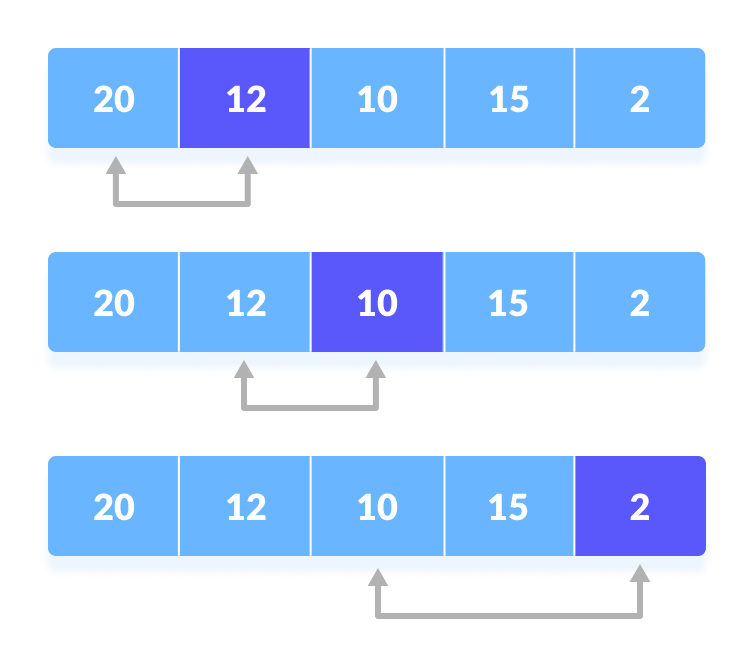
\includegraphics[scale=0.75]{lab8_fig1.png}

            Write a program to do the following:\\\\
            \begin{enumerate}
	
		\item Create an array of 10 random integers.		\\

                \item Sort the array using an algorithm of your choice into {\it greatest to least} order. You will need to describe the algorithm you used in your summary.\\
                
                \item Show the sorted array and the original unsorted array. To do this you must a make a copy before you sort.\\
                
		\item Once you have it working change the array to 100 random integers and verify that is still works.		\\              

                \item \underline{Bonus:} Compare the performance of the two algorithms by timing how long the sorting process takes for each. You can use {\it clock} or {\it tic-toc}. Be sure to start with the same unsorted array for both methods.  
            \end{enumerate}


    \end{description}
 
\newpage


\end{document}



